% -----------------------------------------------------------------------
% executionFlow.tex: Section detailing each of the main algorithms
%                    used by Duchamp.
% -----------------------------------------------------------------------
% Copyright (C) 2006, Matthew Whiting, ATNF
%
% This program is free software; you can redistribute it and/or modify it
% under the terms of the GNU General Public License as published by the
% Free Software Foundation; either version 2 of the License, or (at your
% option) any later version.
%
% Duchamp is distributed in the hope that it will be useful, but WITHOUT
% ANY WARRANTY; without even the implied warranty of MERCHANTABILITY or
% FITNESS FOR A PARTICULAR PURPOSE.  See the GNU General Public License
% for more details.
%
% You should have received a copy of the GNU General Public License
% along with Duchamp; if not, write to the Free Software Foundation,
% Inc., 59 Temple Place, Suite 330, Boston, MA 02111-1307, USA
%
% Correspondence concerning Duchamp may be directed to:
%    Internet email: Matthew.Whiting [at] atnf.csiro.au
%    Postal address: Dr. Matthew Whiting
%                    Australia Telescope National Facility, CSIRO
%                    PO Box 76
%                    Epping NSW 1710
%                    AUSTRALIA
% -----------------------------------------------------------------------
\secA{What \duchamp is doing}
\label{sec-flow}

Each of the steps that \duchamp goes through in the course of its
execution are discussed here in more detail. This should provide
enough background information to fully understand what \duchamp is
doing and what all the output information is. For those interested in
the programming side of things, \duchamp is written in C/C++ and makes
use of the \textsc{cfitsio}, \textsc{wcslib} and \textsc{pgplot}
libraries.

\secB{Image input}
\label{sec-input}

The image cube to be searched is provided to \duchamp in FITS
format. The \texttt{cfitsio} library will read \texttt{.fits} files,
as well as compressed \texttt{.fits.gz} files directly.

The cube is read in using basic \textsc{cfitsio} commands, and stored
as an array in a special C++ class. This class keeps track of the list
of detected objects, as well as any reconstructed arrays that are made
(see \S\ref{sec-recon}). The World Coordinate System
(WCS)\footnote{This is the information necessary for translating the
  pixel locations to quantities such as position on the sky,
  frequency, velocity, and so on.} information for the cube is also
obtained from the FITS header by \textsc{wcslib} functions
\citep{greisen02, calabretta02,greisen06}, and this information, in
the form of a \texttt{wcsprm} structure, is also stored in the same
class. See \S\ref{sec-wcs} for more details.

A sub-section of a cube can be requested by defining the subsection
with the \texttt{subsection} parameter and setting
\texttt{flagSubsection = true} -- this can be a good idea if the cube
has very noisy edges, which may produce many spurious detections.

There are two ways of specifying the \texttt{subsection} string. The
first is the generalised form
\texttt{[x1:x2:dx,y1:y2:dy,z1:z2:dz,...]}, as used by the
\textsc{cfitsio} library. This has one set of colon-separated numbers
for each axis in the FITS file. In this manner, the x-coordinates run
from \texttt{x1} to \texttt{x2} (inclusive), with steps of
\texttt{dx}. The step value can be omitted, so a subsection of the
form \texttt{[2:50,2:50,10:1000]} is still valid. In fact, \duchamp
does not make use of any step value present in the subsection string,
and any that are present are removed before the file is opened.

If the entire range of a coordinate is required, one can replace the
range with a single asterisk, \eg \texttt{[2:50,2:50,*]}. Thus, the
subsection string \texttt{[*,*,*]} is simply the entire cube. Note
that the pixel ranges for each axis start at 1, so the full pixel
range of a 100-pixel axis would be expressed as 1:100. A complete
description of this section syntax can be found at the
\textsc{fitsio} web site%
\footnote{%
\href%
{http://heasarc.gsfc.nasa.gov/docs/software/fitsio/c/c\_user/node91.html}%
{http://heasarc.gsfc.nasa.gov/docs/software/fitsio/c/c\_user/node91.html}}.


Making full use of the subsection requires knowledge of the size of
each of the dimensions. If one wants to, for instance, trim a certain
number of pixels off the edges of the cube, without examining the cube
to obtain the actual size, one can use the second form of the
subsection string. This just gives a number for each axis, \eg
\texttt{[5,5,5]} (which would trim 5 pixels from the start \emph{and}
end of each axis).

All types of subsections can be combined \eg \texttt{[5,2:98,*]}. 

Typically, the units of pixel brightness are given by the FITS file's
BUNIT keyword. However, this may often be unwieldy (for instance, the
units are Jy/beam, but the values are around a few mJy/beam). It is
therefore possible to nominate new units, to which the pixel values
will be converted, by using the \texttt{newFluxUnits} input
parameter. The units must be directly translatable from the existing
ones -- for instance, if BUNIT is Jy/beam, you cannot specify mJy, it
must be mJy/beam. If an incompatible unit is given, the BUNIT value is
used instead.

\secB{World Coordinate System}
\label{sec-wcs}

\duchamp uses the \textsc{wcslib} package to handle the conversions
between pixel and world coordinates. This package uses the
transformations described in the WCS papers
\citep{greisen02,calabretta02,greisen06}. The same package handles the
WCS axes in the spatial plots. The conversions used are governed by
the information in the FITS header -- this is parsed by
\textsc{wcslib} to create the appropriate transformations.

For the spectral axis, however, \duchamp provides the ability to change the
type of transformation used, so that different spectral quantities can
be calculated. By using the parameter \texttt{spectralType}, the user
can change from the type given in the FITS header. This should be done
in line with the conventions outlined in \citet{greisen06}. The
spectral type can be either a full 8-character string (\eg
'VELO-F2V'), or simply the 4-character ``S-type'' (\eg 'VELO'), in
which case \textsc{wcslib} will handle the conversion.

The rest frequency can be provided as well. This may be necessary, if
the FITS header does not specify one and you wish to transform to
velocity. Alternatively, you may want to make your measurements based
on a different spectral line (\eg OH1665 instead of
H\textsc{i}-21cm). The input parameter \texttt{restFrequency} is used,
and this will override the FITS header value.

Finally, the user may also request different spectral units from those
in the FITS file, or from the defaults arising from the
\textsc{wcslib} transformation. The input parameter
\texttt{spectralUnits} should be used, and \citet{greisen02} should be
consulted to ensure the syntax is appropriate.

\secB{Image modification}
\label{sec-modify}

Several modifications to the cube can be made that improve the
execution and efficiency of \duchamp (their use is optional, governed
by the relevant flags in the parameter file).

\secC{BLANK pixel removal}
\label{sec-blank}

If the imaged area of a cube is non-rectangular (see the example in
Fig.~\ref{fig-moment}, a cube from the HIPASS survey), BLANK pixels
are used to pad it out to a rectangular shape. The value of these
pixels is given by the FITS header keywords BLANK, BSCALE and
BZERO. While these pixels make the image a nice shape, they will take
up unnecessary space in memory, and so to potentially speed up the
processing we can trim them from the edge. This is done when the
parameter \texttt{flagTrim = true}. If the above keywords are not
present, the trimming will not be done (in this case, a similar effect
can be accomplished, if one knows where the ``blank'' pixels are, by
using the subsection option).

The amount of trimming is recorded, and these pixels are added back in
once the source-detection is completed (so that quoted pixel positions
are applicable to the original cube). Rows and columns are trimmed one
at a time until the first non-BLANK pixel is reached, so that the
image remains rectangular. In practice, this means that there will be
some BLANK pixels left in the trimmed image (if the non-BLANK region
is non-rectangular). However, these are ignored in all further
calculations done on the cube.

\secC{Negative-feature detection}
\label{sec-negative}

\duchamp searches strictly for positive sources -- that is, pixels
that are \textbf{above} the detection threshold. If one instead wishes
to search for negative features (such as absorption lines), set the
parameter \texttt{flagNegative=true}. 

This inverts the cube (\ie multiplies all pixels by $-1$) prior to
searching, and then re-inverts the cube, and the fluxes of any
detections (so that the detections will have, for instance, a negative
peak flux) after searching is complete. Any reconstructed or smoothed
array that has been read from disk is also inverted. 

This works fine for the simple case of inverting the cube. If,
however, a spectral baseline needs to be removed (see the next section
\S\ref{sec-baseline}), then special care needs to be taken. This is
described in more detail in \S\ref{sec-absorptionline}.

\secC{Baseline removal}
\label{sec-baseline}

The user may request the removal of baselines from the
spectra, via the parameter \texttt{flagBaseline}. This may be
necessary if there is a strong baseline ripple present, which can
result in spurious detections at the high points of the ripple, or if
there is continuum emission present in the cube that is not
interesting for the search.

There are two ways in which the baseline can be calculated. The first
makes use of the \atrous wavelet reconstruction procedure (see
\S\ref{sec-recon}), where only the two largest scales are kept. 

The second method uses a median filter combined with a sliding box of
some specified width. For each pixel, the baseline is determined to be
the median value of all pixels in a region of that width centred on
the pixel of interest. The box is truncated at the edges of the
spectrum (so that fewer pixels are included), but there will always be
at least half the width of the box present.

The choice between these methods is made using the
\texttt{baselineType} parameter -- only values of \texttt{atrous} (the
default) or \texttt{median} are accepted. If the \texttt{median}
method is being used, the full width of the box is specified with
\texttt{baselineBoxWidth}. 

The baseline calculation is done separately for each spatial pixel
(\ie for each spectrum in the cube), and the baselines are stored and
added back in before any output is done. In this way the quoted fluxes
and displayed spectra are as one would see from the input cube itself
-- even though the detection (and reconstruction if applicable) is
done on the baseline-removed cube.

When the \texttt{atrous} method is used, the presence of very strong
signals (for instance, masers at several hundred Jy) could affect the
determination of the baseline, and would lead to a large dip centred
on the signal in the baseline-subtracted spectrum. To prevent this,
the signal is trimmed prior to the reconstruction process at some
standard threshold (at $5\sigma$ above the mean). The baseline
determined should thus be representative of the true, signal-free
baseline. Note that this trimming is only a temporary measure which
does not affect the source-detection.

The baseline values can be saved to a FITS file for later
examination. See \S\ref{sec-baselineOut} for details.

\secC{Combining negative detections with baseline removal}
\label{sec-absorptionline}

When both \texttt{flagNegative=true} and \texttt{flagBaseline=true},
care needs to be taken when parameterising the sources. They are
strictly negative on the baseline-subtracted spectrum, and so
parameterisation is done on this spectrum, prior to adding the
baseline back.

This ensures that the peak flux and location correspond to the maximum
absorption (the peak flux will be quoted as a negative value), and the
spectral plots (see \S\ref{sec-spectralplots}) will properly show the
peak spectrum (when used in \texttt{spectralMethod=peak} mode).

This method is typical of the approach that would be used for
detecting absorption lines against a continuum source. For now, the
parameterisation is the same as for other detections, but a future
version of \duchamp will have parameters more relevant for absorption
lines, such as optical depth and equivalent width.

\secC{Flagging channels}
\label{sec-flagging}

Finally, it is possible to flag particular channels so that they are
not included in the search. This is an extension of the old ``Milky
Way'' channel range. That allowed the specification of a single
contiguous block of channels, and was aimed at excluding Galactic
emission in extragalactic \hi cubes. 

The new flagging approach allows the specification of a series of
channels and channel ranges. This allows the user to block the
detection of known regions of RFI, or known but uninteresting emission
(\eg Galactic \hi emission if you are searching for extragalactic
sources). 

Flagged channels are specified using the \texttt{flaggedChannels}
parameter, and can be given by a comma-separated list of single values
or ranges. For instance: \texttt{flaggedChannels  5,6,12-20,87}. These
channels refer to channel numbers in the \textbf{the full cube},
before any subsection is applied. Also note that \textbf{the channel
  numbering starts at zero}, that is, channel 0 is the first channel
of the cube. 

The effect is to ignore detections that lie within these channels. If
a spatial search is being conducted (\ie one channel map at a time),
these channels are simply not searched. If a spectral search is being
conducted, those channels will be flagged so that no detection is made
within them. The spectral output (see Fig.~\ref{fig-spect}) will
ignore them as far as scaling the plot goes, and the channel range
will be indicated by a green hatched box.

Note that these channels will be included in any smoothing or
reconstruction that is done on the array, and so will be included in
any saved FITS file (see \S\ref{sec-reconIO}).

\secB{Image reconstruction}
\label{sec-recon}

The user can direct \duchamp to reconstruct the data cube using the
multi-resolution \atrous wavelet algorithm. A good description of the
procedure can be found in \citet{starck02a}. The reconstruction is an
effective way of removing a lot of the noise in the image, allowing
one to search reliably to fainter levels, and reducing the number of
spurious detections. This is an optional step, but one that greatly
enhances the reliability of the resulting catalogue, at the cost of
additional CPU and memory usage (see \S\ref{sec-notes} for
discussion).

\secC{Algorithm}

The steps in the \atrous reconstruction are as follows:
\begin{enumerate}
\item The reconstructed array is set to 0 everywhere.
\item The input array is discretely convolved with a given filter
  function. This is determined from the parameter file via the
  \texttt{filterCode} parameter -- see Appendix~\ref{app-param} for
  details on the filters available. Edges are dealt with by assuming
  reflection at the boundary.
\item The wavelet coefficients are calculated by taking the difference
  between the convolved array and the input array.
\item If the wavelet coefficients at a given point are above the
  requested reconstruction threshold (given by \texttt{snrRecon} as
  the number of $\sigma$ above the mean and adjusted to the current
  scale -- see Appendix~\ref{app-scaling}), add these to the
  reconstructed array.
\item The separation between the filter coefficients is doubled. (Note
  that this step provides the name of the procedure\footnote{\atrous
  means ``with holes'' in French.}, as gaps or holes are created in
  the filter coverage.)
\item The procedure is repeated from step 2, using the convolved array
  as the input array.
\item Continue until the required maximum number of scales is reached.
\item Add the final smoothed (\ie convolved) array to the
  reconstructed array. This provides the ``DC offset'', as each of the
  wavelet coefficient arrays will have zero mean.
\end{enumerate}

The range of scales at which the selection of wavelet coefficients is
made is governed by the \texttt{scaleMin} and \texttt{scaleMax}
parameters. The minimum scale used is given by \texttt{scaleMin},
where the default value is 1 (the first scale). This parameter is
useful if you want to ignore the highest-frequency features
(e.g. high-frequency noise that might be present). Normally the
maximum scale is calculated from the size of the input array, but it
can be specified by using \texttt{scaleMax}. A value $\le0$ will
result in the use of the calculated value, as will a value of
\texttt{scaleMax} greater than the calculated value. Use of these two
parameters can allow searching for features of a particular scale
size, for instance searching for narrow absorption features.

The reconstruction has at least two iterations. The first iteration
makes a first pass at the wavelet reconstruction (the process outlined
in the 8 stages above), but the residual array will likely have some
structure still in it, so the wavelet filtering is done on the
residual, and any significant wavelet terms are added to the final
reconstruction. This step is repeated until the relative change in the
measured standard deviation of the residual (see note below on the
evaluation of this quantity) is less than some value, given by the
\texttt{reconConvergence} parameter.

It is important to note that the \atrous decomposition is an example
of a ``redundant'' transformation. If no thresholding is performed,
the sum of all the wavelet coefficient arrays and the final smoothed
array is identical to the input array. The thresholding thus removes
only the unwanted structure in the array.

Note that any BLANK pixels that are still in the cube will not be
altered by the reconstruction -- they will be left as BLANK so that
the shape of the valid part of the cube is preserved.

\secC{Note on Statistics}

The correct calculation of the reconstructed array needs good
estimators of the underlying mean and standard deviation (or rms) of
the background noise distribution. The methods used to estimate these
quantities are detailed in \S\ref{sec-stats} -- the default behaviour
is to use robust estimators, to avoid biasing due to bright pixels.

When thresholding the different wavelet scales, the value of the rms
as measured from the wavelet array needs to be scaled to account for
the increased amount of correlation between neighbouring pixels (due
to the convolution). See Appendix~\ref{app-scaling} for details on
this scaling.

\secC{User control of reconstruction parameters}

The most important parameter for the user to select in relation to the
reconstruction is the threshold for each wavelet array. This is set
using the \texttt{snrRecon} parameter, and is given as a multiple of
the rms (estimated by the MADFM) above the mean (which for the wavelet
arrays should be approximately zero). There are several other
parameters that can be altered as well that affect the outcome of the
reconstruction.

By default, the cube is reconstructed in three dimensions, using a
three-dimensional filter and three-dimensional convolution. This can be
altered, however, using the parameter \texttt{reconDim}. If set to 1,
this means the cube is reconstructed by considering each spectrum
separately, whereas \texttt{reconDim=2} will mean the cube is
reconstructed by doing each channel map separately. The merits of
these choices are discussed in \S\ref{sec-notes}, but it should be
noted that a 2-dimensional reconstruction can be susceptible to edge
effects if the spatial shape of the pixel array is not rectangular.

The user can also select the minimum and maximum scales to be used in
the reconstruction. The first scale exhibits the highest frequency
variations, and so ignoring this one can sometimes be beneficial in
removing excess noise. The default is to use all scales
(\texttt{minscale = 1}).

The convergence of the \atrous iterations is governed by the
\texttt{reconConvergence} parameter, which is the fractional decrease
in the standard deviation of the residuals from one iteration to the
next. \duchamp will do at least two iterations, and then continue
until the decrease is less than the value of this parameter.

Finally, the filter that is used for the convolution can be selected
by using \texttt{filterCode} and the relevant code number -- the
choices are listed in Appendix~\ref{app-param}. A larger filter will
give a better reconstruction, but take longer and use more memory when
executing. When multi-dimensional reconstruction is selected, this
filter is used to construct a 2- or 3-dimensional equivalent.

\secB{Smoothing the cube}
\label{sec-smoothing}

An alternative to doing the wavelet reconstruction is to smooth the
cube.  This technique can be useful in reducing the noise level (at
the cost of making neighbouring pixels correlated and blurring any
signal present), and is particularly well suited to the case where a
particular signal size (\ie a certain channel width or spatial size)
is believed to be present in the data.

There are two alternative methods that can be used: spectral
smoothing, using the Hanning filter; or spatial smoothing, using a 2D
Gaussian kernel. These alternatives are outlined below. To utilise the
smoothing option, set the parameter \texttt{flagSmooth=true} and set
\texttt{smoothType} to either \texttt{spectral} or \texttt{spatial}.

\secC{Spectral smoothing}

When \texttt{smoothType = spectral} is selected, the cube is smoothed
only in the spectral domain. Each spectrum is independently smoothed
by a Hanning filter, and then put back together to form the smoothed
cube, which is then used by the searching algorithm (see below). Note
that in the case of both the reconstruction and the smoothing options
being requested, the reconstruction will take precedence and the
smoothing will \emph{not} be done.

There is only one parameter necessary to define the degree of
smoothing -- the Hanning width $a$ (given by the user parameter
\texttt{hanningWidth}). The coefficients $c(x)$ of the Hanning filter
are defined by
\[
c(x) = 
  \begin{cases}
   \frac{1}{2}\left(1+\cos(\frac{\pi x}{a})\right) &|x| < (a+1)/2\\
   0                                               &|x| \geq (a+1)/2.
  \end{cases},\ a,x \in \mathbb{Z}
\]
Note that the width specified must be an
odd integer (if the parameter provided is even, it is incremented by
one).

\secC{Spatial smoothing}

When \texttt{smoothType = spatial} is selected, the cube is smoothed
only in the spatial domain. Each channel map is independently smoothed
by a two-dimensional Gaussian kernel, put back together to form the
smoothed cube, and used in the searching algorithm (see below). Again,
reconstruction is always done by preference if both techniques are
requested.

The two-dimensional Gaussian has three parameters to define it,
governed by the elliptical cross-sectional shape of the Gaussian
function: the FWHM (full-width at half-maximum) of the major and minor
axes, and the position angle of the major axis. These are given by the
user parameters \texttt{kernMaj, kernMin} \& \texttt{kernPA}. If a
circular Gaussian is required, the user need only provide the
\texttt{kernMaj} parameter. The \texttt{kernMin} parameter will then
be set to the same value, and \texttt{kernPA} to zero.  If we define
these parameters as $a,b,\theta$ respectively, we can define the
kernel by the function
\[ 
k(x,y) = \frac{1}{2\pi\sigma_X\sigma_Y} \exp\left[-0.5
  \left(\frac{X^2}{\sigma_X^2} + \frac{Y^2}{\sigma_Y^2} \right)
\right]
\]
where $(x,y)$ are the offsets from the central pixel of the gaussian
function, and 
\begin{align*}
X& = x\sin\theta - y\cos\theta&
  Y&= x\cos\theta + y\sin\theta\\
\sigma_X^2& = \frac{(a/2)^2}{2\ln2}&
  \sigma_Y^2& = \frac{(b/2)^2}{2\ln2}\\
\end{align*}

The size of the kernel is determined both by these FWHM parameters and
the cutoff parameter \texttt{spatialSmoothCutoff}. The width is
determined by 
\[
W = \sigma_\text{maj} \sqrt{(2\log(C))}
\]
where $C$ is the cutoff value. The value of $W$ is rounded up to get
the half-width of the kernel in pixels. The default value of
\texttt{spatialSmoothCutoff} is 1.e-10, which gives full kernel widths
of 31 pix for \texttt{kernMaj=5} and 19 pix for \texttt{kernMaj=3}. 

The algorithm provides different ways, controlled by the input
parameter \texttt{smoothEdgeMethod}, to handle those pixels that lie
within a kernel half-width from the edge of the image and so cannot
have the full kernel placed on top of them. The default behaviour,
with \texttt{smoothEdgeMethod=equal}, simply treats these pixels in
the same way, adding up the product of the kernel pixels with the
image pixels for all cases that lie within the image boundary. A more
drastic alternative, \texttt{smoothEdgeMethod=truncate}, is to simply
not evaluate the convolution at these pixels -- they will be set at
some null value that will not contribute to any detection. Thirdly,
setting \texttt{smoothEdgeMethod=scale} will evaluate the convolution
as for the \texttt{'equal'} case, but scale down the edge pixels by
summing over only those kernel pixels contributing.

\secB{Input/Output of reconstructed/smoothed arrays}
\label{sec-reconIO}

The smoothing and reconstruction stages can be relatively
time-consuming, particularly for large cubes and reconstructions in
3-D (or even spatial smoothing). To get around this, \duchamp provides
a shortcut to allow users to perform multiple searches (\eg with
different thresholds) on the same reconstruction/smoothing setup
without re-doing the calculations each time.

To save the reconstructed array as a FITS file, set
\texttt{flagOutputRecon = true}. The file will be saved in the same
directory as the input image, so the user needs to have write
permissions for that directory.

The name of the file can given by the \texttt{fileOutputRecon}
parameter, but this can be ignored and \duchamp will present a name
based on the reconstruction parameters. The filename will be derived
from the input filename, with extra information detailing the
reconstruction that has been done. For example, suppose
\texttt{image.fits} has been reconstructed using a 3-dimensional
reconstruction with filter \#2, thresholded at $4\sigma$ using all
scales from 1 to 5, with a convergence criterion of 0.005. The output
filename will then be \texttt{image.RECON-3-2-4-1-5-0.005.fits} (\ie
it uses the six parameters relevant for the \atrous reconstruction as
listed in Appendix~\ref{app-param}). The new FITS file will also have
these parameters as header keywords. If a subsection of the input
image has been used (see \S\ref{sec-input}), the format of the output
filename will be \texttt{image.sub.RECON-3-2-4-1-5-0.005.fits}, and the
subsection that has been used is also stored in the FITS header.

Likewise, the residual image, defined as the difference between the
input and reconstructed arrays, can also be saved in the same manner
by setting \texttt{flagOutputResid = true}. Its filename will be the
same as above, with \texttt{RESID} replacing \texttt{RECON}.

If a reconstructed image has been saved, it can be read in and used
instead of redoing the reconstruction. To do so, the user should set
the parameter \texttt{flagReconExists = true}. The user can indicate
the name of the reconstructed FITS file using the \texttt{reconFile}
parameter, or, if this is not specified, \duchamp searches for the
file with the name as defined above. If the file is not found, the
reconstruction is performed as normal. Note that to do this, the user
needs to set \texttt{flagAtrous = true} (obviously, if this is
\texttt{false}, the reconstruction is not needed).

To save the smoothed array, set \texttt{flagOutputSmooth = true}. As
for the reconstructed/residual arrays, the name of the file can given
by the parameter \texttt{fileOutputSmooth}, but this can be ignored
and \duchamp will present a name that indicates the both the type and
the details of the smoothing method used. It will be either
\texttt{image.SMOOTH-1D-a.fits}, where a is replaced by the Hanning
width used, or \texttt{image.SMOOTH-2D-a-b-c-X-f.fits}, where a,b,c
are the Gaussian kernel parameters, X represents the edge method
(E=equal, T=truncate, S=scale), and f is
$-\log_{10}(\text{cutoff})$. Similarly to the reconstruction case, a
saved file can be read in by setting \texttt{flagSmoothExists = true}
and either specifying a file to be read with the \texttt{smoothFile}
parameter or relying on \duchamp to find the file with the name as
given above.


\secB{Searching the image}
\label{sec-detection}

\secC{Representation of detected objects}
\label{sec-scan}

\begin{figure}[t]
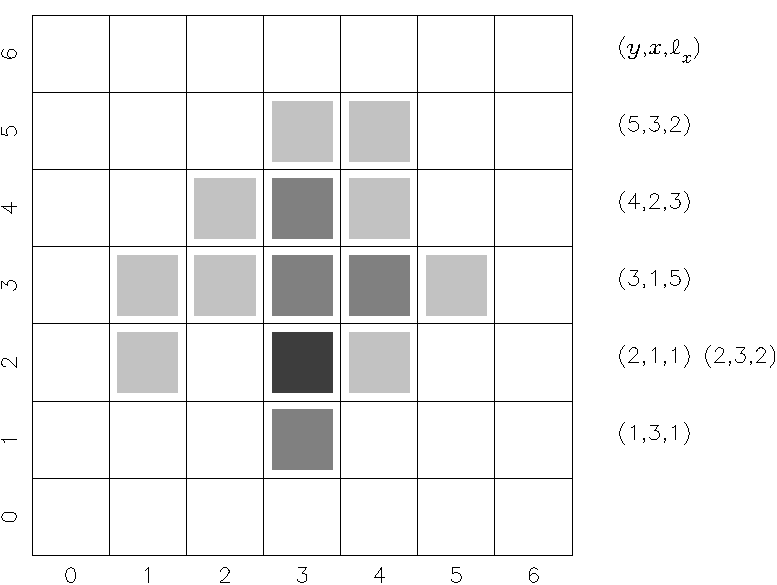
\includegraphics[width=\textwidth]{exampleObject}
\caption{An example of the run-length encoding method of storing
pixel information. The scans used to encode the image are listed
alongside the relevant row. The pixels are colour-coded by
nominal pixel values, but note that the pixel values themselves
do not form part of the encoding and are not kept as part of the
object class. }
\label{fig-objExample}
\end{figure}

The principle aim of \duchamp is to provide a catalogue of sources
located in the image. While running, \duchamp needs to maintain for
each source several data structures that will contribute to the memory
footprint: a record of which pixels contribute to the source; a set of
measured parameters that will go into the catalogue; and a separate
two-dimensional map showing the spatial location of detected pixels
(carrying this around makes the computation of detection maps easier
-- see \S\ref{sec-spatialmaps}).

To keep track of the set of detected pixels, \duchamp
employs specialised techniques that keep the memory usage
manageable. A naive method could be to store each single pixel, but
this results in a lot of redundant information being stored in memory.

To reduce the storage requirements, the run-length encoding method is
used for storing the spatial information. In this fashion, an object
in 2D is stored as a series of ``runs'', encoded by a row number (the
$y$-value), the starting column (the minimum $x$-value) and the run
length ($\ell_x$: the number of contiguous pixels in that row
connected to the starting pixel). A single set of $(y,x,\ell_x)$
values is called a ``scan''. A two-dimensional image is therefore made
up of a set of scans. An example can be seen in
Fig.~\ref{fig-objExample}. Note that the object shown has fourteen
pixels, and so would require 28 integers to record the positions of
all pixels. The run-length encoding uses just 18 integers to record
the same information. The longer the runs are in each scan, the
greater the saving of storage over the naive method.

A 3D object is stored as a set of channel maps, with a channel map
being a 2D plane with constant $z$-value. Each channel map is itself a
set of scans showing the $(x,y)$ position of the pixels. The
additional detection map is stored as a separate channel map, also
made up of scans.

Note that these pixel map representations do not carry the flux
information with them. They store just the pixel locations and need to
be combined with an array of flux values to provide parameters such as
integrated flux. The advantage of this approach is that the pixel
locations can be easily applied to different flux arrays as the need
permits (for instance, defining them using the reconstructed array,
yet evaluating parameters on the original array).

This scan-based run-length encoding is how the individual detections
are stored in the binary catalogue described in \S\ref{sec-bincat}.

\secC{Technique}
\label{sec-searchTechnique}

The basic idea behind detection in \duchamp is to locate sets of
contiguous voxels that lie above some threshold. No size or shape
requirement is imposed upon the detections, and no fitting (for
instance, fitting Gaussian profiles) is done on the sources. All
\duchamp does is find connected groups of bright voxels and report
their locations and basic parameters.

One threshold is calculated for the entire cube, enabling calculation
of signal-to-noise ratios for each source (see
\S\ref{sec-output} for details). The user can manually specify a
value (using the parameter \texttt{threshold}) for the threshold,
which will override the calculated value. Note that this option
overrides any settings of \texttt{snrCut} or FDR options (see below).

The cube can be searched in one of two ways, governed by the input
parameter \texttt{searchType}. If \texttt{searchType=spatial}, the
cube is searched one channel map at a time, using the 2-dimensional
raster-scanning algorithm of \citet{lutz80} that connects groups of
neighbouring pixels. Such an algorithm cannot be applied directly to a
3-dimensional case, as it requires that objects are completely nested
in a row (when scanning along a row, if an object finishes and other
starts, you won't get back to the first until the second is completely
finished for the row). Three-dimensional data does not have this
property, hence the need to treat the data on a 2-dimensional basis at
most.

Alternatively, if \texttt{searchType=spectral}, the searching is done
in one dimension on each individual spatial pixel's spectrum. This is
a simpler search, but there are potentially many more of them.

Although there are parameters that govern the minimum number of pixels
in a spatial, spectral and total sense that an object must have
(\texttt{minPix}, \texttt{minChannels} and \texttt{minVoxels}
respectively), these criteria are not applied at this point - see
\S\ref{sec-reject} for details.

Finally, the search only looks for positive features. If one is
interested instead in negative features (such as absorption lines),
set the parameter \texttt{flagNegative = true}. This will invert the
cube (\ie multiply all pixels by $-1$) prior to the search, and then
re-invert the cube (and the fluxes of any detections) after searching
is complete. If the reconstructed or smoothed array has been read in
from disk, this will also be inverted at the same time. All outputs
are done in the same manner as normal, so that fluxes of detections
will be negative.

\secC{Calculating statistics}
\label{sec-stats}

A crucial part of the detection process (as well as the wavelet
reconstruction: \S\ref{sec-recon}) is estimating the statistics that
define the detection threshold. To determine a threshold, we need to
estimate from the data two parameters: the middle of the noise
distribution (the ``noise level''), and the width of the distribution
(the ``noise spread''). The noise level is estimated by either the
mean or the median, and the noise spread by the rms (or the standard
deviation) or the median absolute deviation from the median
(MADFM). The median and MADFM are robust statistics, in that they are
not biased by the presence of a few pixels much brighter than the
noise.

All four statistics are calculated automatically, but the choice of
parameters that will be used is governed by the input parameter
\texttt{flagRobustStats}. This has the default value \texttt{true},
meaning the underlying mean of the noise distribution is estimated by
the median, and the underlying standard deviation is estimated by the
MADFM. In the latter case, the value is corrected, under the
assumption that the underlying distribution is Normal (Gaussian), by
dividing by 0.6744888 -- see Appendix~\ref{app-madfm} for details. If
\texttt{flagRobustStats=false}, the mean and rms are used instead.

The choice of pixels to be used depend on the analysis method. If the
wavelet reconstruction has been done, the residuals (defined
in the sense of original $-$ reconstruction) are used to estimate the
noise spread of the cube, since the reconstruction should pick out
all significant structure. The noise level (the middle of the
distribution) is taken from the original array.

If smoothing of the cube has been done instead, all noise parameters
are measured from the smoothed array, and detections are made with
these parameters. When the signal-to-noise level is quoted for each
detection (see \S\ref{sec-output}), the noise parameters of the
original array are used, since the smoothing process correlates
neighbouring pixels, reducing the noise level.

If neither reconstruction nor smoothing has been done, then the
statistics are calculated from the original, input array. 

The parameters that are estimated should be representative of the
noise in the cube. For the case of small objects embedded in many
noise pixels (\eg the case of \hi surveys), using the full cube will
provide good estimators. It is possible, however, to use only a
subsection of the cube by setting the parameter \texttt{flagStatSec =
  true} and providing the desired subsection to the \texttt{StatSec}
parameter. This subsection works in exactly the same way as the pixel
subsection discussed in \S\ref{sec-input}. The \texttt{StatSec} will
be trimmed if necessary so that it lies wholly within the image
subsection being used (\ie that given by the \texttt{subsection}
parameter - this governs what pixels are read in and so are able to be
used in the calculations).

Note that \texttt{StatSec} applies only to the statistics used to
determine the threshold. It does not affect the calculation of
statistics in the case of the wavelet reconstruction. Note also that
pixels identified as BLANK or as flagged via the
\texttt{flaggedChannels} parameter are ignored in the statistics
calculations.

\secC{Determining the threshold}

Once the statistics have been calculated, the threshold is determined
in one of two ways. The first way is a simple sigma-clipping, where a
threshold is set at a fixed number $n$ of standard deviations above
the mean, and pixels above this threshold are flagged as detected. The
value of $n$ is set with the parameter \texttt{snrCut}. The ``mean''
and ``standard deviation'' here are estimated according to
\texttt{flagRobustStats}, as discussed in \S\ref{sec-stats}. In this
first case only, if the user specifies a threshold, using the
\texttt{threshold} parameter, the sigma-clipped value is ignored.

The second method uses the False Discovery Rate (FDR) technique
\citep{miller01,hopkins02}, whose basis we briefly detail here. The
false discovery rate (given by the number of false detections divided
by the total number of detections) is fixed at a certain value
$\alpha$ (\eg $\alpha=0.05$ implies 5\% of detections are false
positives). In practice, an $\alpha$ value is chosen, and the ensemble
average FDR (\ie $\langle FDR \rangle$) when the method is used will
be less than $\alpha$.  One calculates $p$ -- the probability,
assuming the null hypothesis is true, of obtaining a test statistic as
extreme as the pixel value (the observed test statistic) -- for each
pixel, and sorts them in increasing order. One then calculates $d$
where
\[
d = \max_j \left\{ j : P_j < \frac{j\alpha}{c_N N} \right\},
\]
and then rejects all hypotheses whose $p$-values are less than or
equal to $P_d$. (So a $P_i<P_d$ will be rejected even if $P_i \geq
j\alpha/c_N N$.) Note that ``reject hypothesis'' here means ``accept
the pixel as an object pixel'' (\ie we are rejecting the null
hypothesis that the pixel belongs to the background).

The $c_N$ value here is a normalisation constant that depends on the
correlated nature of the pixel values. If all the pixels are
uncorrelated, then $c_N=1$. If $N$ pixels are correlated, then their
tests will be dependent on each other, and so $c_N = \sum_{i=1}^N
i^{-1}$. \citet{hopkins02} consider real radio data, where the pixels
are correlated over the beam. For the calculations done in \duchamp,
$N = B \times C$, where $B$ is the beam area in pixels, calculated
from the FITS header (if the correct keywords -- BMAJ, BMIN -- are not
present, the size of the beam is taken from the input parameters - see
discussion in \S\ref{sec-results}, and if these parameters are not
given, $B=1$), and $C$ is the number of neighbouring channels that can
be considered to be correlated.

The use of the FDR method is governed by the \texttt{flagFDR} flag,
which is \texttt{false} by default. To set the relevant parameters,
use \texttt{alphaFDR} to set the $\alpha$ value, and
\texttt{FDRnumCorChan} to set the $C$ value discussed above. These
have default values of 0.01 and 2 respectively.

The theory behind the FDR method implies a direct connection between
the choice of $\alpha$ and the fraction of detections that will be
false positives. These detections, however, are individual pixels,
which undergo a process of merging and rejection (\S\ref{sec-merger}),
and so the fraction of the final list of detected objects that are
false positives will be much smaller than $\alpha$. See the discussion
in \S\ref{sec-notes}.

%\secC{Storage of detected objects in memory}
%
%It is useful to understand how \duchamp stores the detected objects in
%memory while it is running. This makes use of nested C++ classes, so
%that an object is stored as a class that includes the set of detected
%pixels, plus all the various calculated parameters (fluxes, WCS
%coordinates, pixel centres and extrema, flags,...). The set of pixels
%are stored using another class, that stores 3-dimensional objects as a
%set of channel maps, each consisting of a $z$-value and a
%2-dimensional object (a spatial map if you like). This 2-dimensional
%object is recorded using ``run-length'' encoding, where each row (a
%fixed $y$ value) is stored by the starting $x$-value and the length

\secB{Merging, growing and rejecting detected objects}
\label{sec-merger}

\secC{Merging}

The searches described above are either 1- or 2-dimensional only. They
do not know anything about the third dimension that is likely to be
present. To build up 3D sources, merging of detections must be
done. This is done via an algorithm that matches objects judged to be
``close'', according to one of two criteria.

One criterion is to define two thresholds -- one spatial and one in
velocity -- and say that two objects should be merged if there is at
least one pair of pixels that lie within these threshold distances of
each other. These thresholds are specified by the parameters
\texttt{threshSpatial} and \texttt{threshVelocity} (in units of pixels
and channels respectively).

Alternatively, the spatial requirement can be changed to say that
there must be a pair of pixels that are \emph{adjacent} -- a stricter,
but perhaps more realistic requirement, particularly when the spatial
pixels have a large angular size (as is the case for \hi
surveys). This method can be selected by setting the parameter
\texttt{flagAdjacent=true} in the parameter file. The velocity
thresholding is always done with the \texttt{threshVelocity} test. 


\secC{Stages of merging}

This merging can be done in two stages. The default behaviour is for
each new detection to be compared with those sources already detected,
and for it to be merged with the first one judged to be close. No
other examination of the list is done at this point.

This step can be turned off by setting
\texttt{flagTwoStageMerging=false}, so that new detections are simply
added to the end of the list, leaving all merging to be done in the
second stage.

The second, main stage of merging is more thorough, Once the searching
is completed, the list is iterated through, looking at each pair of
objects, and merging appropriately. The merged objects are then
included in the examination, to see if a merged pair is suitably close
to a third.

\secC{Growing}

Once the detections have been merged, they may be ``grown'' (this is
essentially the process known elsewhere as ``floodfill''). This is a
process of increasing the size of the detection by adding nearby
pixels (according to the \texttt{threshSpatial} and
\texttt{threshVelocity} parameters) that are above some secondary
threshold and not already part of a detected object. This threshold
should be lower than the one used for the initial detection, but above
the noise level, so that faint pixels are only detected when they are
close to a bright pixel. This threshold is specified via one of two
input parameters. It can be given in terms of the noise statistics via
\texttt{growthCut} (which has a default value of $3\sigma$), or it can
be directly given via \texttt{growthThreshold}. Note that if you have
given the detection threshold with the \texttt{threshold} parameter,
the growth threshold \textbf{must} be given with
\texttt{growthThreshold}. If \texttt{growthThreshold} is not provided
in this situation, the growing will not be done.

The use of the growth algorithm is controlled by the
\texttt{flagGrowth} parameter -- the default value of which is
\texttt{false}. If the detections are grown, they are sent through the
merging algorithm a second time, to pick up any detections that should
be merged at the new lower threshold (\ie they have grown into each
other). 

\secC{Rejecting}
\label{sec-reject}

Finally, to be accepted, the detections must satisfy minimum (and,
optionally, maximum) size criteria, relating to the number of
channels, spatial pixels and voxels occupied by the object. These
criteria are set using the \texttt{minChannels}, \texttt{minPix} and
\texttt{minVoxels} parameters respectively. The channel requirement
means a source must have at least one set of \texttt{minChannels}
consecutive channels to be accepted. The spatial pixels
(\texttt{minPix}) requirement refers to distinct spatial pixels (which
are possibly in different channels), while the voxels requirement
refers to the total number of voxels detected. If the
\texttt{minVoxels} parameter is not provided, it defaults to
\texttt{minPix}$+$\texttt{minChannels}-1.

It is possible to also place upper limits on the size of detections in
a similar fashion. The corresponding parameters are \texttt{maxPix},
\texttt{maxChannels} and \texttt{maxVoxels}. These will all default to
a value of -1 -- if they are negative the check is \textbf{not}
made. If they are provided by the user, an object will be rejected if
one of the metrics exceeds the limit (in each case, the value is the
highest allowed value for an object to be accepted). The channel
requirement differs slightly from the minimum check -- the limit
applies to the total number of channels in the object.

It is possible to do this rejection stage before the main merging and
growing stage. This could be done to remove narrow (hopefully
spurious) sources from the list before growing them, to reduce the
number of false positives in the final list. This mode can be selected
by setting the input parameter \texttt{flagRejectBeforeMerge=true} --
caution is urged if you use this in conjunction with
\texttt{flagTwoStageMerging=false}, as you can throw away parts of
objects that you may otherwise wish to keep.

%%% Local Variables: 
%%% mode: latex
%%% TeX-master: "Guide"
%%% End: 
